\section{Davide Alpi}
La mia responsabilità principale è stata l'implementazione della view del gioco.

Per prima cosa motiverò la mia scelta della libreria grafica (libGDX).
In seguito, descriverò il package "scalagdx", un layer che ho creato on top di libGDX per semplificarne e renderne più idiomatico l'utilizzo.
Infine, illustrerò l'interazione tra la view e l'ActorSystem, con seguente zoom sul ViewActor.


\subsection{Libreria grafica}
\label{sec:view}

Le librerie grafiche che ho valutato per lo sviluppo della parte di View sono state:
\begin{itemize}
    \item ScalaFX: la libreria più usata all'interno dell'ecosistema Scala per la creazione di interfacce grafiche
    \item Indigo: libreria Scala per la creazione di giochi
    \item libGDX: la libreria Java ad alto livello più usata per la creazione di giochi
\end{itemize}
Verrà scelta la tecnologia tenendo conto dei seguenti parametri:
\begin{itemize}
    \item Qualità della documentazione: La documentazione è completa e aggiornata? Gli esempi forniti compilano? 
    \item Adozione: quanti progetti, commerciali e non, sono stati completati con questa tecnologia?
    \item Query results: numero di risultati di query google relative a diverse problematiche che gli sviluppatori tipicamente devono affrontare durante l'utilizzo della libreria.
    \item Funzionalità: quanto permette di fare? Quanto è vasta e flessibile l'API fornita?
\end{itemize}

\subsubsection{Indigo}
Indigo è stata subito scartata perchè nessun progetto commerciale è ancora stato completato con il suo utilizzo (livello di adozione troppo basso). Anche gli altri parametri non raggiungono livelli soddisfacenti.

\subsubsection{ScalaFX}
ScalaFX, pur essendo la libreria Scala più utilizzata per la creazione di interfacce grafiche, rimane una libreria Scala, e pertanto il suo grado di adozione è limitato.
La documentazione è molto scarna e alcuni esempi contenuti non buildano.

\subsubsection{libGDX - scelta finale}
Una miriade di progetti commerciali sono stati portati avanti con libGDX. La sua API nel corso degli ultimi 5 anni ha subito poche sostanziali modifiche, evidenziando un importante grado di maturità raggiunto. Essendo una libreria Java, il numero di query result è esponenzialmente maggiore rispetto alle altre scelte.

Da un punto di vista commerciale, libGDX è la scelta migliore.
Anche da un punto di vista di ricerca, è interessante capire come libGDX può essere inserito all'interno di un progetto Scala in maniera idiomatica. Si sfrutta anche la possibilità di Scala di accedere all'intero ecosistema Java. Per questa serie di motivazioni, ho scelto libGDX come libreria grafica.

\subsection{scalagdx}
\subsubsection{Screen}
libGDX fornisce un'API che permette di definire in maniera piuttosto imperativa il codice da "agganciare" all'esecuzione di alcuni "lifecylcle methods" delle schermate di gioco (ScreenAdapter).
Un esempio è il metodo "render", metodo dello ScreenAdapter che verrà chiamato dal motore grafico ad ogni frame. Effettuandone l'override, è possibile quindi definire cosa disegnare a schermo ciascun frame. L'implementazione di diversi ScreenAdapter è tediosa, error-prone, e richiede una grande quantità di boilerplate code.

Con scalagdx.Screen.ScreenBehavior ho voluto risolvere questo problema, fornendo un'API per definire in maniera più dichiarativa gli elementi che dovranno apparire a schermo. Lo ScreenBehavior si basa anche sui concetti di Drawable e Writable objects, che modellano rispettivamente delle immagini e delle scritte unitamente ai loro boundaries all'interno del viewport.

\begin{lstlisting}[language=Scala, label=code:screen-behavior, caption=trait ScreenBehavior]
  trait ScreenBehavior:
    def drawables: Seq[Drawable]
    def writables: Seq[Writable]
    def actors: Seq[Actor]
    def onScreenTouch: Vector2 => Unit
    def viewport: Viewport
\end{lstlisting}

\begin{figure}[H]
    \centering
    \caption{ScreenBehavior's promise of execution}
    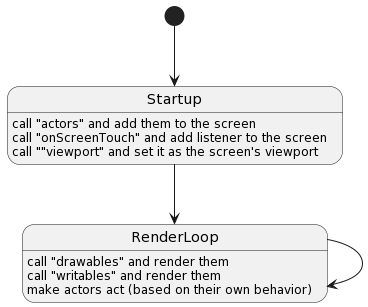
\includegraphics[width=0.8\linewidth]{sections/images/screen-behavior.png}
    \label{ScreenBehavior}
\end{figure}


Lo ScreenBehavior può essere poi usato per costruire un BasicScreen, che implementa ScreenAdapter. Lo ScreenBehavior può anche essere convertito implicitamente in BasicScreen grazie al meccanismo delle given conversion.


\subsubsection{Clickable}
Il mio obiettivo era attuare il pattern "pimp my library" per aggiungere un metodo "onTouchDown" e "onTouchUp" alle classi di libGDX "Actor" e "Stage".
Entrambi implementano il metodo "addListener" (con la stessa signature), ma non hanno sfortunatamente interfacce comuni da poter estendere (con extension method ad esempio).
Una soluzione sarebbe stata implementare extension methods per entrambe le classi per implementare i due metodi di cui sopra per entrambe le classi. Questo avrebbe portato però alla duplicazione del codice.

La soluzione adottata è stata la seguente:

\begin{lstlisting}[language=Scala, label=code:clickable, caption=trait Clickable]
  trait Clickable:
    protected def addListener(cl: EventListener): Boolean
    def onTouchDown(f: Vector2 => Unit): Unit = addListener(new ClickListener :
      override def touchDown(event: InputEvent, x: Float, y: Float, pointerId: Int, buttonId: Int): Boolean =
        super.touchDown(event, x, y, pointerId, buttonId)
        f(Vector2(x, y))
        true
    )
    def onTouchUp(f: () => Unit): Unit = addListener(new ClickListener :
      override def touchUp(event: InputEvent, x: Float, y: Float, pointerId: Int, buttonId: Int): Unit =
        super.touchUp(event, x, y, pointerId, buttonId)
        f()
    )
    
  given Conversion[Actor, Clickable] = actor => new Clickable :
    export actor.addListener

  given Conversion[Stage, Clickable] = stage => new Clickable :
    export stage.addListener
\end{lstlisting}

Il trait Clickable implementa le funzionalità aggiuntive in comune tra tutte le classi che implementano "addListener" (in questo caso "Actor" e "Stage".

\subsubsection{ImageButton builder}
Per semplificare l'istanziamento di ImageButton, e ridurre la necessità di boilerplate code, ho realizzato il seguente builder.

\begin{lstlisting}[language=Scala, label=code:image-buttons, caption=Builder pattern per ImageButtons]

object ImageButtons:
  case class ImageButtonBuilder private[ImageButtons](source: Texture|ImageButtonStyle, bounds: Rectangle = Rectangle(0, 0, 0, 0)):
    def withBounds(x: Float, y: Float, width: Float, height: Float): ImageButtonBuilder = copy(bounds = Rectangle(x, y, width, height))

    def build: ImageButton =
      val button = source match
        case t: Texture => ImageButton(TextureRegionDrawable(t))
        case s: ImageButtonStyle => ImageButton(s)
      button.setBounds(bounds.x, bounds.y, bounds.width, bounds.height)
      button.setTransform(true)
      button

  def withSource(source: Texture|ImageButtonStyle): ImageButtonBuilder = ImageButtonBuilder(source)

  given Conversion[ImageButtonBuilder, ImageButton] = _.build
  
\end{lstlisting}

Grazie alla given conversion, è possibile evitare la chiamata finale al "build()" e rendere così il suo utilizzo più fluente:

\begin{lstlisting}[language=Scala, label=code:image-buttons-example, caption=Esempio di creazione di un ImageButton con e senza given conversion abilitata]

val source: Texture = ???

ImageButtons.withSource(source).withBounds(0,0,0,0).build()

import ImageButtons.given

ImageButtons withSource source withBounds (0,0,0,0)

\end{lstlisting}

Questo builder pattern potrebbe essere implementato anche per molte altre classi di libGDX che si intendono usare, seguendo lo stesso schema.
Nel caso degli ImageButton, una source è obbligatoria per la creazione dell'oggetto, ma in caso il builder non richieda parametri obbligatori basta cambiare il metodo "withSource(...)" in un generico "builder".


\subsection{Game}

\subsubsection{Lancio dell'applicazione}
Una volta sviluppato il \textit{core} di un'applicazione con libGDX, occorre definire un \textit{main} ad hoc per ciascuna piattaforma che si intende supportare. Ho creato quindi un launcher con LWJGL3 per supportare i dispositivi desktop.

Al launcher LWJGL3 deve essere fornita una particolare classe di libGDX. Ho implementato quindi un'estensione di questa classe, "\textbf{Game}", che rappresenta l'entry point del \textit{core} della nostra applicazione. 

Il Game agisce da top level controller dell'applicazione, occupandosi di avviare l'ActorSystem ogni volta che viene avviata una nuova partita e cambiando schermata quando richiesto.

\subsubsection{Interazione tra Game e ActorSystem}
Di seguito le interazioni tra il Game e l'ActorSystem (che contiene, tra gli altri attori, il ViewActor).
Sono mostrate anche le tre schermate di gioco, implementate con MainMenuScreen, GameScreen e GameOverScreen.


\begin{figure}[H]
    \centering
    \caption{Interazioni di lancio applicazione, inizio partita e fine partita}
    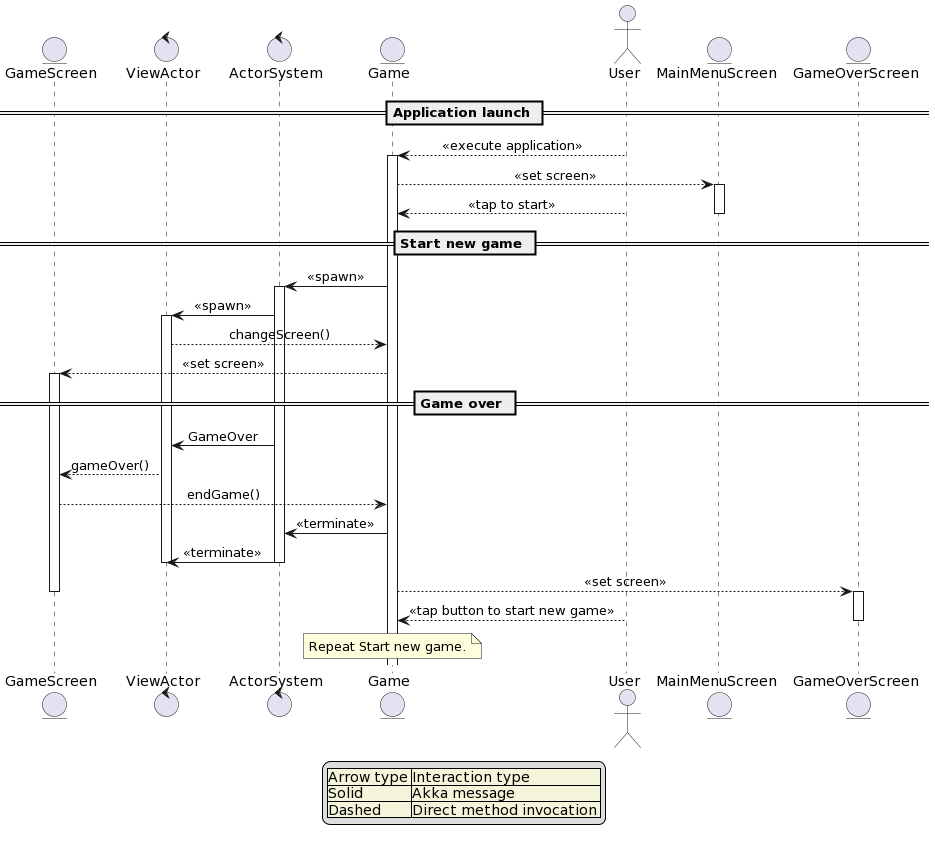
\includegraphics[width=0.8\linewidth]{sections/images/actors-game-interaction.png}
    \label{ScreenBehavior}
\end{figure}


\subsubsection{ViewActor}
Il ViewActor rappresenta la parte di View dell'ActorSystem, come illustrato nel capitolo relativo al Design di Dettaglio. Il seguente diagramma di sequenza mostra come ho gestito le interazioni tra esso e il GameScreen.

\begin{figure}[H]
    \centering
    \caption{ViewActor message exchange during game}
    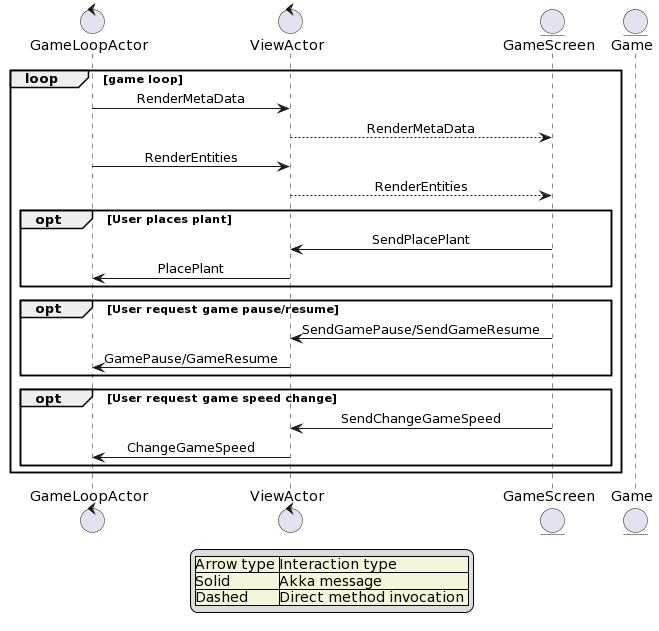
\includegraphics[width=0.8\linewidth]{sections/images/view-actor.png}
    \label{ScreenBehavior}
\end{figure}

